\documentclass {article}

\usepackage{graphicx}
\usepackage{multicol}
\usepackage{hyperref} 

\usepackage{amsmath}
\begin{document}
	
	
	%
	%Title template { Title } {Workplace } {Name/date }
	%\newcommand{\waterlootitle}[3]{
	%\begin{singlespace}
	% \begin{titlepage}
	%
	%  \begin{center}
	
	% \textbf{\MakeUppercase{ University of Waterloo }} \\
	% \textbf{Faculty of Mathematics}
	
	% \vfill  
	
	%{
	% \large
	%\textsc{\textbf{\textit{#1}}}
	% }
	
	%  \vfill
	
	%#2
	
	%\vfill
	
	%prepared by \\[1em]
	%#3
	
	%\end{center}
	
	%\end{titlepage}
	%\end{singlespace}
	%}
	%
	
	%~\vfill
	\begin{center}
		\Large
		
		\textbf{\MakeUppercase{CSC2521 - Computational Design and Fabrication Fall 2017}}
		\vfill  
		
		{
			\Huge
			\textbf{Assignment 2}
		}
		
		{
			\Large
			\textsc{\textbf{Parametric Design}}
		}
		
		\vfill
		Name: Lawson Fulton
		
		Student ID: 998262062
		
		October 13, 2017
	\end{center}
	
	\newpage
	\noindent{\Large \bf Results:}
	\begin{description}
		\item[Basic Functionality]:\\
		
		Originally I wanted to make a twisty menger sponge, but that turned out to be too much of a pain. So instead, it's just a twisted menger sponge of depth 1 that can be tiled. The main parameters are \texttt{twist\_degrees}, the degrees that the box twists. \texttt{hole\_scale}, the scale of the hole relative to the box. And \texttt{n\_wide, n\_long, n\_tall} for the number of repetitions in each direction.
		
		\begin{figure*}[ht!]
			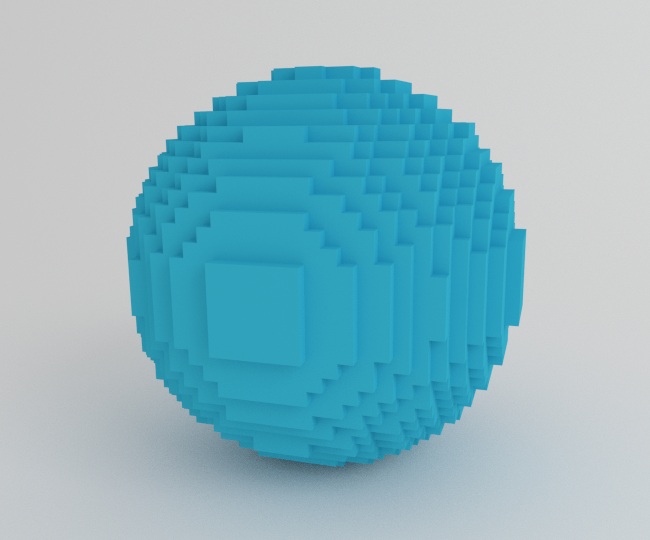
\includegraphics[width=.3\textwidth]{../data/renders/sphere32}\hfill
			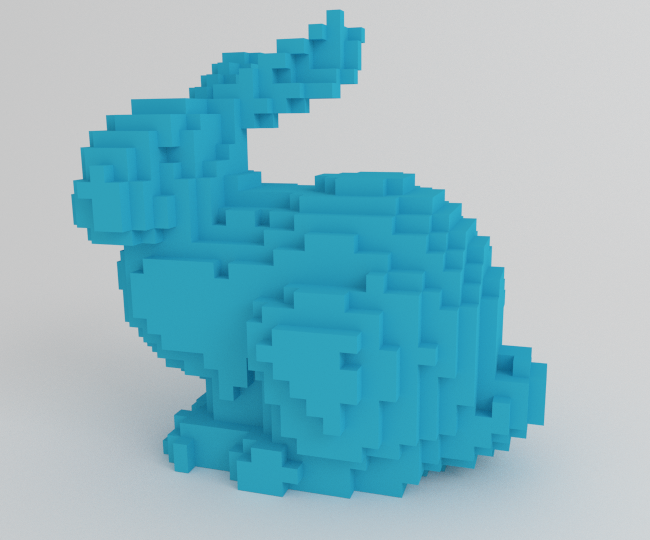
\includegraphics[width=.3\textwidth]{../data/renders/bunny32}\hfill
			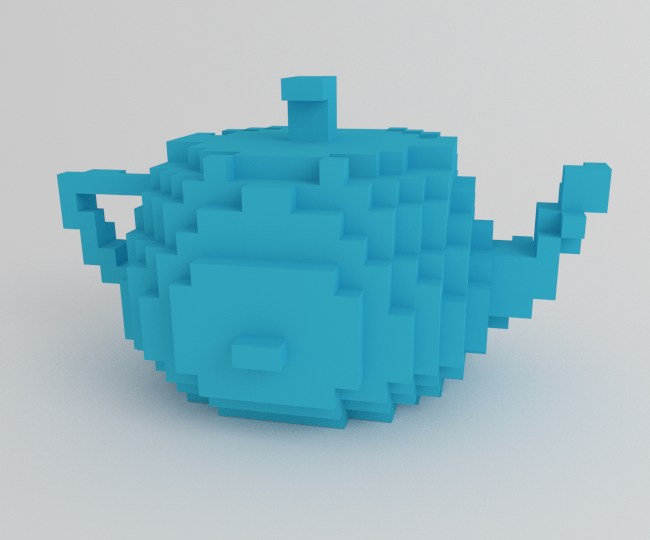
\includegraphics[width=.3\textwidth]{../data/renders/teapot32}
			\caption{34x34x34}
		\end{figure*}
		
		\newpage

		\item[Sources]:\\
		
		1. Fast algorithm for ray-triangle intersection: \href{http://en.wikipedia.org/wiki/M%C3%B6ller%E2%80%93Trumbore_intersection_algorithm}{Moller-Trumbore intersection algorithm}. 
		
		2. Branchless ray to bounding-box intersection algorithm: \href{http://tavianator.com/2011/05/fast-branchless-raybounding-box-intersections/}{http://tavianator.com/2011/05/fast-branchless-raybounding-box-intersections/}.  
		
		3. Stanford 3D scanning repository for Stanford dragon mesh: \href{http://graphics.stanford.edu/data/3Dscanrep/}{http://graphics.stanford.edu/data/3Dscanrep/}. 
		
	\end{description}
	
\end{document}
